\documentclass[twocolumn,pra,amsmath,amssymb,superscriptaddress,longbibliography,nofootinbib,floatfix]{revtex4-2}
\usepackage[utf8]{inputenc}
\usepackage{pgfplots}
\usepackage[colorlinks=true, linkcolor=red, allbordercolors={white}]{hyperref}
\pgfplotsset{compat = newest}
\usepgfplotslibrary{colorbrewer}
\usepgfplotslibrary{groupplots}
\usetikzlibrary{arrows.meta}
\pgfplotsset{
  cycle list={color1\\color2\\color3\\color4\\color5\\color6\\color7\\color8\\color9\\},
}
\tikzset{
    new dash/.code args={on #1 off #2}{
        % Use csname so catcode of @ doesn't have do be changed.
        \csname tikz@addoption\endcsname{%
            \pgfgetpath\currentpath%
            \pgfprocessround{\currentpath}{\currentpath}%
            \csname pgf@decorate@parsesoftpath\endcsname{\currentpath}{\currentpath}%
            \pgfmathparse{\csname pgf@decorate@totalpathlength\endcsname-#1}\let\rest=\pgfmathresult%
            \pgfmathparse{#1+#2}\let\onoff=\pgfmathresult%
            \pgfmathparse{max(floor(\rest/\onoff), 1)}\let\nfullonoff=\pgfmathresult%
            \pgfmathparse{max((\rest-\onoff*\nfullonoff)/\nfullonoff+#2, #2)}\let\offexpand=\pgfmathresult%
            \pgfsetdash{{#1}{\offexpand}}{0pt}}%
    }
}

\begin{document}

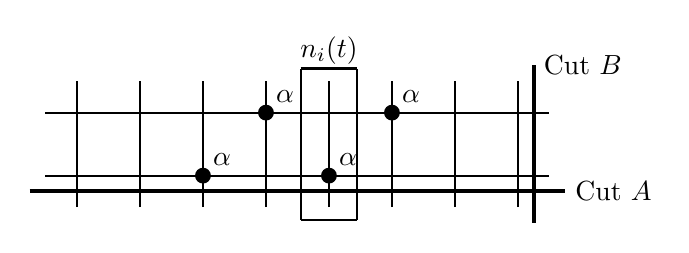
\begin{tikzpicture}[line width=0.75pt, scale=0.8]
	\draw[black] (-4.5,0) -- (3.5,0);
	\draw[black] (-4.5,1) -- (3.5,1);
	\draw[black] (-4,-0.5) -- (-4,1.5);
	\draw[black] (-3,-0.5) -- (-3,1.5);
	\draw[black] (-2,-0.5) -- (-2,1.5);
	\draw[black] (-1,-0.5) -- (-1,1.5);
	\draw[black] (0,-0.5) -- (0,1.5);
	\draw[black] (1,-0.5) -- (1,1.5);
	\draw[black] (2,-0.5) -- (2,1.5);
	\draw[black] (3,-0.5) -- (3,1.5);
	\draw[black][line width=1.5pt] (3.25,-0.75) -- (3.25,1.75);
	\node[black, anchor=west] (a) at (3.25,1.75) {Cut $B$};
	\draw[black][line width=1.5pt] (-4.75,-0.25) -- (3.75,-0.25);
	\node[black, anchor=west] (a) at (3.75,-0.25) {Cut $A$};
	\node[draw,circle,inner sep=1.75pt,fill,black] at (-1,1) {};
	\node[draw,circle,inner sep=1.75pt,fill,black] at (-2,0) {};
	\node[draw,circle,inner sep=1.75pt,fill,black] at (0,0) {};
	\node[draw,circle,inner sep=1.75pt,fill,black] at (1,1) {};
	\node[black, anchor=south west] (a) at (-1,1) {$\alpha$};
	\node[black, anchor=south west] (a) at (-2,0) {$\alpha$};
	\node[black, anchor=south west] (a) at (0,0) {$\alpha$};
	\node[black, anchor=south west] (a) at (1,1) {$\alpha$};
	\draw[black] (0.45,-0.7) -- (0.45,1.7);
	\draw[black] (-0.45,-0.7) -- (-0.45,1.7);
	\draw[black] (-0.45,1.7) -- (0.45,1.7);
	\draw[black] (-0.45,-0.7) -- (0.45,-0.7);
	\node[black, anchor=south] (a) at (0,1.6) {$n_i(t)$};
\end{tikzpicture}

\end{document}